\documentclass[11pt,a4paper]{article}

\usepackage[utf8]{inputenc}
\usepackage[english]{babel}
\usepackage[T1]{fontenc}

\usepackage{amsmath,amssymb,amsfonts}
\usepackage{hyperref}

\usepackage{graphicx}
\usepackage{subcaption}
\usepackage{caption}

\title{Computational Geometry - Visibility Graphs and Motion Planning}
\author{Philip Munksgaard \\ Sebastian Paaske Tørholm \\ Ejnar Håkonsen}

\begin{document}
\maketitle

\section{Exercise 13.4}

We have implemented the algorithm in Mathematica. The resulting drawings
can be seen in \autoref{ex13.4}.

\begin{figure}
    \centering
    \begin{subfigure}[b]{.4\textwidth}
        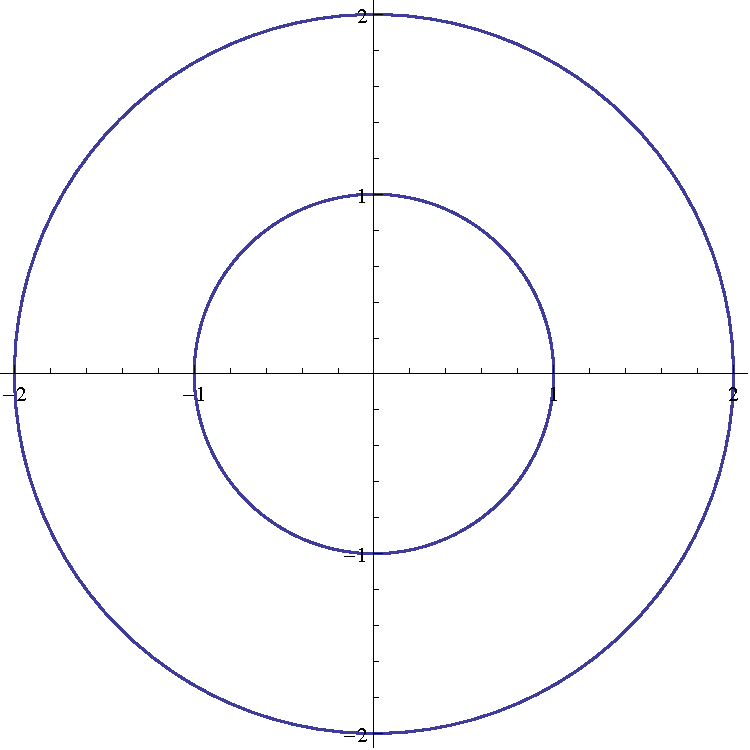
\includegraphics[width=\textwidth]{ex13-4-a.pdf}
        \caption{13.4 a}
    \end{subfigure}
    \begin{subfigure}[b]{.4\textwidth}
        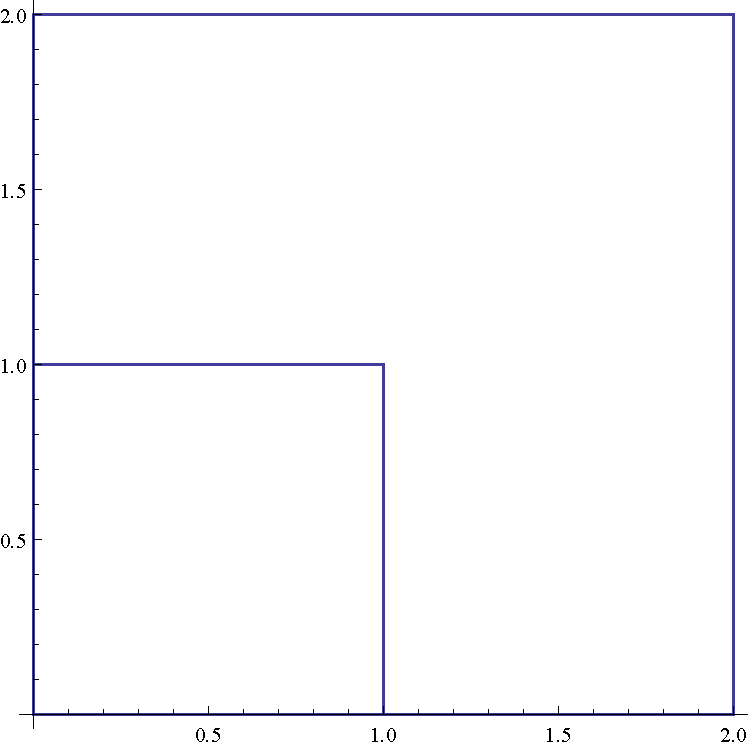
\includegraphics[width=\textwidth]{ex13-4-b.pdf}
        \caption{13.4 b}
    \end{subfigure}
    \\
    \begin{subfigure}[b]{.4\textwidth}
        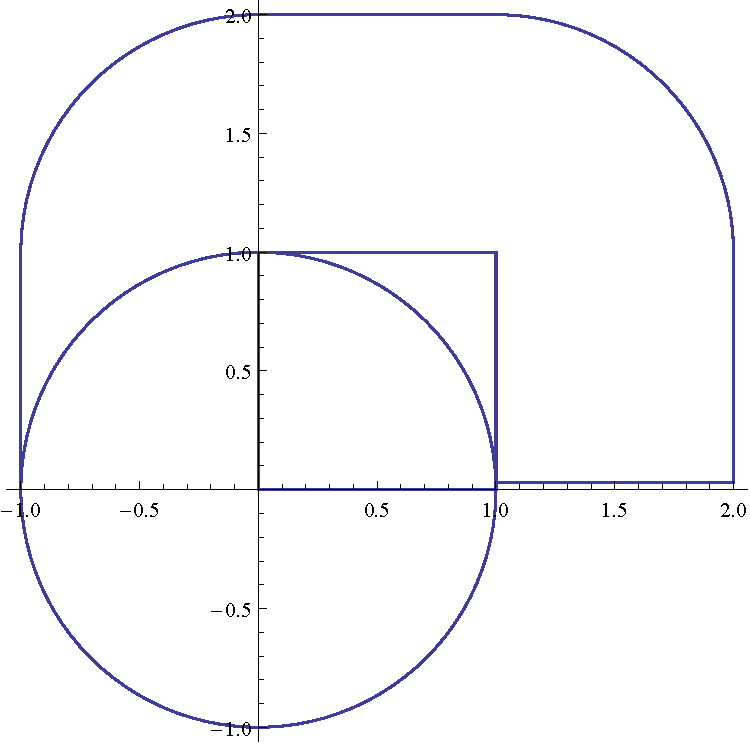
\includegraphics[width=\textwidth]{ex13-4-c.pdf}
        \caption{13.4 c}
    \end{subfigure}
    \begin{subfigure}[b]{.4\textwidth}
        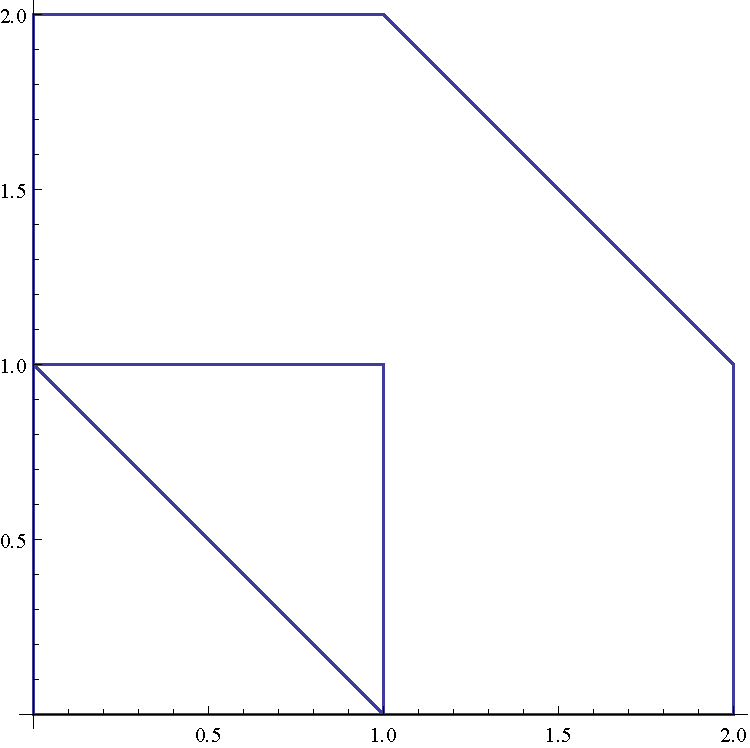
\includegraphics[width=\textwidth]{ex13-4-d.pdf}
        \caption{13.4 d}
    \end{subfigure}
    \caption{The Minkowski sums for exercise 13.4}
    \label{ex13.4}
\end{figure}

\section{Exercise 15.5}

We proceed with the preprocessing as in the algorithm for
\verb+ShortestPath+. However, when using Dijkstra's algorithm, we
continue to iterate through the whole graph and save the shortest path
from $p_{start}$ to all other vertices in the graph.

Then, if we want to compute the shortest path from $p_{start}$ to some
other point $p_{goal}$, we first use \verb+VisibleVertices+ to compute
the set of visible vertices from $p_{goal}$. Then we find the visible
vertice $v$ with the shortest distance from $p_{goal}$. Finally, we
look up the shortest path from $p_{start}$ to $v$, to find the total
shortest path from $p_{start}$ to $p_{goal}$.

Preprocessing takes $O(n^2 \log n)$ time. We can even save the
shortest paths in an array, since lookup is allowed to take $O(n \log
n)$. Finding the set of visible vertices around $p_{goal}$ takes $O(n
\log n)$, finding the closest vertice takes $O(n)$, and looking up the
shortest path from $p_{start}$ to that vertice takes $O(n)$.

\end{document}
